The Australian Ovarian Cancer Study (AOCS)\cite{Patch_2015} performed whole genome sequencing on 92 high grade serous Ovarian cancer tumors, including 15 donors with matched primary and acquired resistance samples. Their analysis found that the recurrence samples harbored more somatic mutations than the primary samples and were enriched for mutations in a $C(C \gt T)C$ context, suggestive of a possible impact of chemotherapy. We extend this analysis by quantifying the number of potential neoantigen-generating mutations in the primary and recurrence samples and testing whether mutational signature deconvolution attributes the unique-to-recurrence mutations to the \texit{C. Elegans} cisplatin signature. We include three additional donors from TCGA and one donor from our institution in our analysis (\ref{tab:cohort}).

Ideally we would have some non-chemo treated surigical patients to serve as control. As platinum chemo is standard of care, we have to use signatures to figure out if it's likely due to chemo.

As surgery is not usually performed for relapsed disease, the AOCS relapsed samples consist predominantly of drained ascites samples. We analyze ascites separately from solid tumors to avoid confounding.



\section*{Results}

\subsection*{Change in mutations and neoantigens at recurrence}
In a Bayesian model integrating both paired and unpaired samples, the post-treatment timepoint was associated with a 49\% (95\% credible region $-2--125$) increase in somatic mutations. There was a 90\% posterior probability that treatment was associated with a meaningful increase in mutations. These results are in basic agreement with non-Bayesian paired and unpaired analysis of this data.

We identified 20,672 potential neoantigens, defined as mutated peptides predicted to bind autologous MHC class I with affinity $\leq 500$nm (Table \ref{tab:cohort}). All but 29 (0.14\%) neoantigens were private to a single donor. The number of neoantigens tracked the increase in mutational burden at relapse. In the Bayesian analysis, treated samples had 49\% (-19--182) more neoantigens, and, for ascites samples, 104\% (2--300) more expressed neoantigens. Interestingly, sold tumor samples showed an increase in neoantigens but a decrease in expressed neoantigens.

% Across the 115 samples from 93 donors, w

\subsection*{Mutation signatures}
We deconvolved each sample's mutations into the 30 mutational signatures curated by COSMIC (http://cancer.sanger.ac.uk/cosmic/signatures), plus four additional signatures extracted from a study of cisplatin-exposed \textit{C. Elegans} [Meier et al], and a chicken cell line exposed to cisplatin, cyclophosphamide, and etoposide\cite{Szikriszt_2016}. The active signatures were largely the same in pre- and post-treatment samples. In both groups, the top signatures were \textit{Signature 3}, associated with BRCA disruption and accounting for 37\% (bootstrap 95\% CI 34-39) of mutations, \textit{Signature 8}, of unknown etiology and accounting for 19\% (17-20) of mutations, and \textit{Signature 1}, associated with age at diagnosis and accounting for 10\% (8-11) of mutations. The remaining mutations were attributed to different signatures in various samples. No samples showed presence of either cisplatin signature or the etoposide signature, but two pre-treatment and five post-treatment samples had evidence for the cyclophosphamide signature.

For better sensitivity to detect signatures operative at relapse, we next focused on the 12 donors with paired pre- and post-treatment samples. We extracted the mutations that had evidence only in the 14 treated samples from these donors. We used a stringent read filter, requiring coverage in both pre- and post-treatment samples and zero variant reads in the pre-treatment samples, including RNA when available. Of $229,132$ SNV mutations in the relapse samples for these donors, we identified $106,171$ ``unique to treated'' mutations, which we then used in signature deconvolution. Two samples (AOCS-092-13, AOCS-095-13) showed evidence for the chicken cisplatin signature. All four donors (AOCS-064, AOCS-093, AOCS-137, AOCS-139) with a clinical record of cyclophophamide treatment showed evidence for the chicken cyclophosphamide signature. However, five donors (AOCS-086, AOCS-088, AOCS-091, AOCS-092, AOCS-095) without a  record of cyclophosphamide use also exhibited this signature. \textit{Signature 1} was completely absent, consistent with its association with slow ongoing mutagenic processes present in all tissue. All samples showed \textit{Signature 3} (BRCA disruption), and 9 of 14 samples showed \textit{Signature 8} (unknown etiology), indicating that the processes likely play a role in the continued evolution post-treatment. Other signatures appeared only sporadically.

\subsection*{Multinucleotide variants and indels}


\section*{Discussion}

The fraction of cancer cells harboring a neoantigen may be critical in its ability to be targeted by a T cell response \cite{McGranahan_2016}.

The loss of expressed neoantigens in the solid tumors is interesting. Consistent with increased immune surveillence.

The loss of 

\section*{Limitations}
RNA with hard thresholds to detect expressed peptides is subject to confounding by changes in gene expression -- e.g. if something gets upregulated post treatment

\section*{Figures and Tables}

\begin{table}
\begin{tabular}{llllll}
\toprule
{} & donors & samples (RNA) &            Mutations &    Neoantigens & Expressed neoantigens \\
\midrule
ascites untreated      &      4 &         4 (4) &   10336 (9600-11000) &  205 (140-270) &           82 (50-110) \\
ascites post-treatment &     22 &       25 (20) &  13757 (12000-15000) &  303 (260-350) &         149 (120-180) \\
solid untreated        &     75 &       75 (69) &     7902 (7000-8900) &  166 (140-190) &            70 (58-83) \\
solid post-treatment   &      9 &        12 (5) &   11250 (8400-14000) &  335 (220-460) &            41 (29-52) \\
\bottomrule
\end{tabular}

\caption{Cohort size and means.}
\label{tab:cohort}
\end{table}

\begin{figure}
\centering
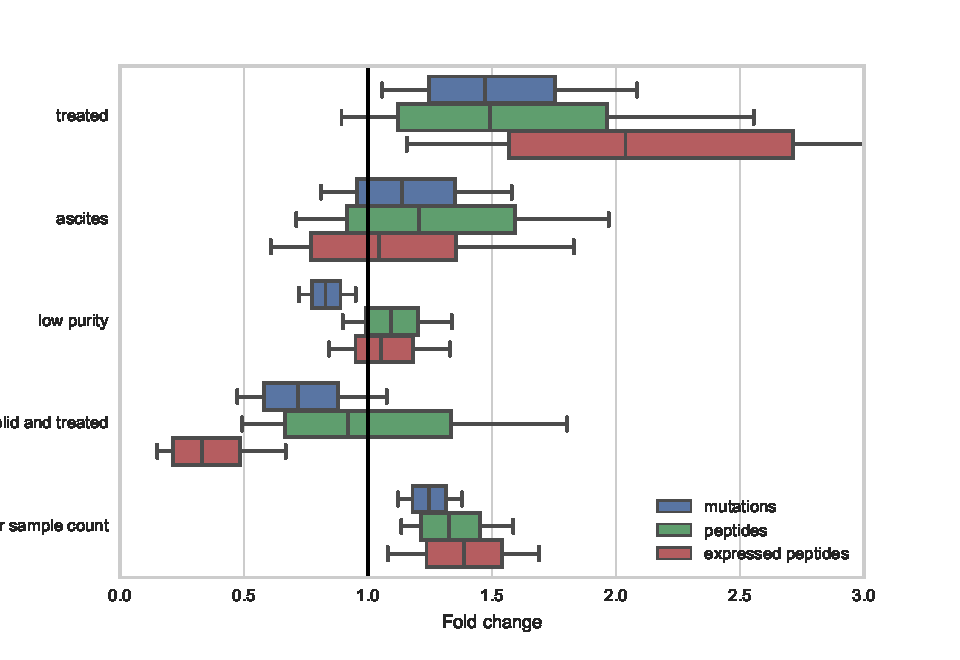
\includegraphics[scale=1.0]{figures/bayesian_model_effects.pdf}
\caption{Bayesian model effects. }
\label{fig:bayesian}
\end{figure}

\begin{figure}
\centering
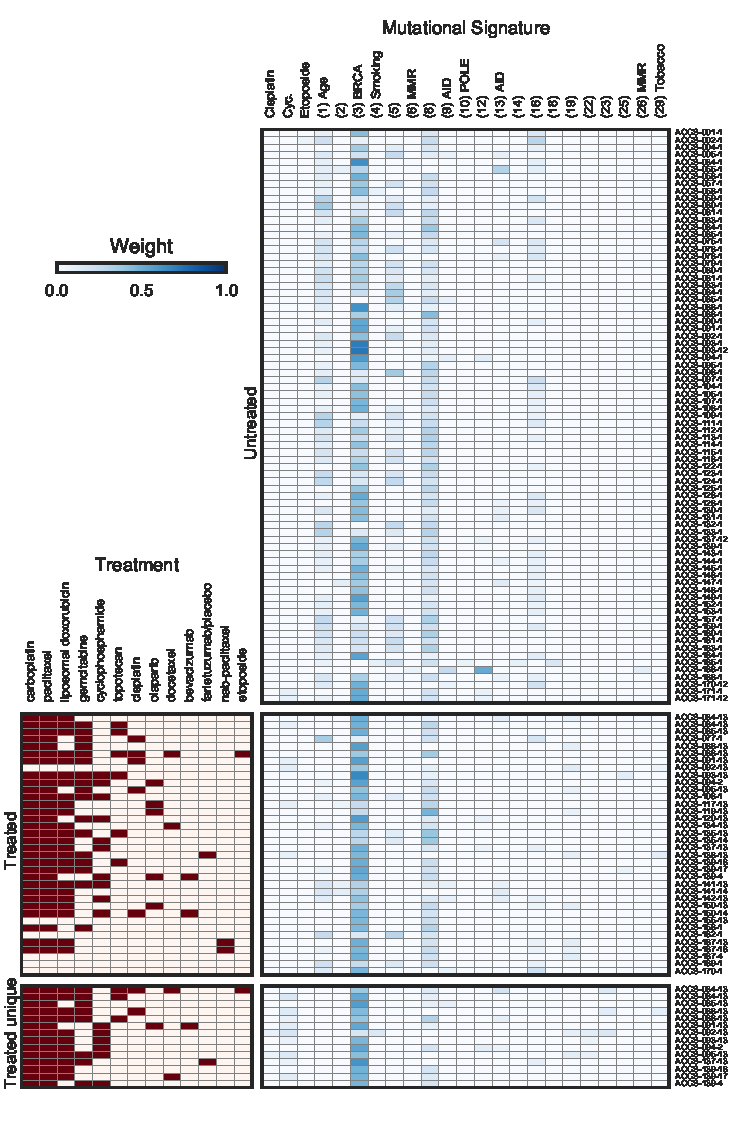
\includegraphics[scale=1.0]{figures/signatures.pdf}
\caption{Mutational signature deconvolution. }
\label{fig:signature}
\end{figure}


Methods
 - Bayesian: used a ROPE of 5\%
 This model integrated information from paired pre- and post-treatment samples and unpaired samples, controlling for sample tissue type (solid or ascites), sample purity, the number of samples from each donor, and allowing for an interaction (effect modification) between tissue type and 
